\documentclass[a4paper]{article}
\usepackage{titling}
\usepackage{authblk}
\usepackage{fancyhdr}
\usepackage{hyperref}
\usepackage{rsc}
\usepackage{siunitx}
\usepackage{graphicx}
\usepackage{listings}
\usepackage{color}

\definecolor{dkgreen}{rgb}{0,0.6,0}
\definecolor{gray}{rgb}{0.5,0.5,0.5}
\definecolor{mauve}{rgb}{0.58,0,0.82}


\lstset{frame=tb,
  language=Python,
  aboveskip=3mm,
  belowskip=3mm,
  showstringspaces=false,
  columns=flexible,
  basicstyle={\ttfamily},
  numbers=none,
  numberstyle=\tiny\color{gray},
  keywordstyle=\color{blue},
  commentstyle=\color{dkgreen},
  stringstyle=\color{mauve},
  breaklines=true,
  breakatwhitespace=true,
  tabsize=3
}
\DeclareSIUnit\Fahrenheit{\degree F}
\setlength{\parindent}{0pt}
\parskip 1.5ex

\title{Lecture 2: Lists, loops, arrays, and plotting}
\author[1]{Dr Benjamin J. Morgan}
\author[1,2]{Dr Andrew R. McCluskey}
\affil[1]{Department of Chemistry, University of Bath, email: b.j.morgan@bath.ac.uk}
\affil[2]{Diamond Light Source, email: andrew.mccluskey@diamond.ac.uk}
\setcounter{Maxaffil}{0}
\renewcommand\Affilfont{\itshape\small}

\pagestyle{fancy}
\fancyhf{}
\rhead{CH40208}
\lhead{\thetitle}
\rfoot{\thepage}

\begin{document}
\maketitle

\section*{Aim}
This week introduces \textbf{lists}, which provide one way to store and manipulate collections of values or variables; \textbf{loops}, which allow you to perform repeated actions; \textbf{numpy arrays}, which provide a compact way to work efficiently with lists of numbers; and \textbf{matplotlib}, which can be used for plotting graphs.

\section{Lists}
A \textbf{list} is an ordered collection of objects, and is created using square brackets \texttt{[ $\ldots$ ]}, with objects separated by commas \texttt{,}.
\begin{lstlisting}
# Making a list

elements = ["Hydrogen", "Helium", "Lithium", "Beryllium", "Boron", "Carbon", "Nitrogen", "Oxygen"]
\end{lstlisting}
A list can contain just one, or even zero objects, with a length-zero list called an ``empty'' list.
\begin{lstlisting}
# A list containing only one element

one_element = ["Hydrogen"]
\end{lstlisting}
\begin{lstlisting}
# An empty list

zero_elements = []
\end{lstlisting}
Individual elements of a list can be referenced using the list's variable name followed by square brackets containing the element's \textbf{index}, e.g.\ \texttt{elements[2]} to return \texttt{"Lithium"}:
\begin{lstlisting}
# Printing some items

print(elements[0])
print(elements[4])
print(elements[-1])
\end{lstlisting}
Python indexing starts from \texttt{0} for the first element of the list, and finishes at \texttt{n-1} for the final element in a list of length $n$. You can also use \textbf{negative indexing} to count backwards from the end, such as \texttt{elements[-1]} in the previous example.
\begin{figure}[tb]
  \centering
  \resizebox{12cm}{!}{\includegraphics*{list_indexing.pdf}} %
    \caption{\label{fig:list_indexing}Schematic of the \texttt{elements} list, showing normal and negative indices for each element.}
\end{figure}
Elements in lists can be treated as normal variables, including assigning them new values using \texttt{=}
\begin{lstlisting}
# Assigning an element of a list to a new value

elements[3] = "Sausage"
print(elements)
elements[3] = "Beryllium"
print(elements)
\end{lstlisting}

As well as referencing individual list elements, you can reference a subset of elements using \textbf{list slicing}. A slice is obtained by providing two index values in the form \texttt{start:end}, e.g.
\begin{lstlisting}
# Select three elements

print(elements[1:4])
\end{lstlisting}
In this example we get a sublist containing three items. This behaviour might seem odd at first, because we asked for elements ``1 to 4'', but is clearer to see when thinking about how lists are normally indexed in Python (see Figure~\ref{fig:list_slicing}). Another way to think about this is that there are 3 elements between indices 1 and 4 ($4-1=3$).
\begin{figure}[tb]
  \centering
  \resizebox{12cm}{!}{\includegraphics*{list_slicing.pdf}} %
    \caption{\label{fig:list_slicing}List slicing.}
\end{figure}
You can select non-consecutive objects from a list by explicitly providing all indices, separated by commas,
\begin{lstlisting}
# Just the gases

print(elements[0, 1, 6, 7])
\end{lstlisting}
Objects can be added to the end of a list using the \texttt{append} operation,
\begin{lstlisting}
# Add more to the list

elements.append("Fluorine")
elements.append("Neon")
print(elements)
\end{lstlisting}
and can be deleted using \texttt{del},
\begin{lstlisting}
# Deleting from a list

del elements[9]
print(elements)
\end{lstlisting}
If two lists need to be combined, this can be achieved by \emph{concatenation},
\begin{lstlisting}
# Concatenating lists
list1 = [1, 4, 6, 2]
list2 = [3, 5, 2]

print(list1 + list2)
\end{lstlisting}
More operations that may be performed on lists can be found at \url{https://docs.python.org/3/tutorial/datastructures.html}.

Data stored in lists do not all need to have the same type.
For example, the list below contains a \texttt{float}, two \texttt{str}, a \texttt{complex} number and an \texttt{int},
\begin{lstlisting}
# List of many types

a_new_list = ['hello', 12.41242, 5 + 8j, 'sadness', 2]
print(a_new_list)
\end{lstlisting}
\vspace{\baselineskip}
\begin{center}
	\noindent\fbox{%
		\begin{minipage}{0.9\textwidth}%
			\vspace{0.15\baselineskip}
			\subsubsection*{Exercise}
			\begin{itemize}
				\item{Create two lists, one containing names the first 8 elements in the periodic table and another containing the masses of those elements. Then, using a loop, print each element name and mass number, format each print statment with the \texttt{.format()} syntax.}
			\end{itemize}
		\end{minipage}
	}
\end{center}

\section{Loops}

Often we want to perform the same computational operation multiple times. One way to do this is to use \textbf{loops}. Python provides two types of loop:
\begin{itemize}
	\item{\texttt{for} loops iterate through a given sequence.}
	\item{\texttt{while} loops continue to repeat, as long as a specific condition is \texttt{True}.}
\end{itemize}
The following examples show a \texttt{for} loop and a \texttt{while} loop, both being used to sum the numbers 1 to 5:
\begin{lstlisting}
# using a "for" loop

total = 0
for n in [1, 2, 3, 4, 5]:
    print(n)
    total = total + n
print('using a for loop: {}'.format(total))
\end{lstlisting}
\begin{lstlisting}
# using a "while" loop

total = 0
n = 1
while n <= 5:
    print(n)
    total = total + n
    n = n + 1
print('using a while loop: {}'.format(total))
\end{lstlisting}
In the first example, using \texttt{for}, we explicitly loop over every element in a list \texttt{[1, 2, 3, 4, 5]}. For each iteration the variable \texttt{n} is set to \texttt{0}, then \texttt{1}, then \texttt{2}, and so on, until we reach the end of the list. The code that we want to repeat is indented below the \texttt{for} statement. In this case we print the current value of \texttt{n} and add it to our total. After the final iteration of the loop, we continue to the next line \emph{outside} the loop, indicated by resetting the indentation at the start of the lines, and print our total.

In the second example, we have used a \texttt{while} statement to specify the condition for continuing to repeat the loop. In this case, the condition is that \texttt{n} is less or equal to 5. Inside the loop (again indicated by the indented lines) we print the current value of \texttt{n}, and add it to our total, but also increment \texttt{n} by one. If this line was left out, \texttt{n} would never change from the initial value of 1, and the loop would continue an infinite number of times.

In the first example, we can replace the list \texttt{[0, 1, 2, 3, 4, 5]} with a \texttt{range}
\begin{lstlisting}
# using a "for" loop and "range"

total = 0
for n in range(1,5):
    print(n)
    total = total + n
print('using a "for" loop: {}'.format(total))
\end{lstlisting}
The \texttt{range} function generates a sequence of integers that we can iterate over, similar to iterating over elements of a list.

In the second example, a more compact way to write \texttt{n = n + 1} (add one to the value stored in \texttt{n} and store the new value in \texttt{n}) is to instead write \texttt{n += 1} (increment the value stored in \texttt{n} by 1).
\begin{lstlisting}
# using a "while" loop and "+=" to increment a variable

total = 0
n = 1
while n <= 5:
    print(n)
    total = total + n
    n += 1
print('using a "while" loop: {}'.format(total))
\end{lstlisting}

In the code below we iterate though the first ten chemical element symbols and print each one.
\begin{lstlisting}
# Printing the periodic table

elements = ["H", "He", "Li", "Be", "B", "C", "N", "O", "F", "Ne"]

for symbol in elements:
	print(symbol)
\end{lstlisting}
If we want to count the index of these elements as we loop over them, without doing it manually (e.g.\ using \texttt{i += 1}) we can use the \texttt{enumerate} function:
\begin{lstlisting}
# Using enumerate in a for loop

for i, symbol in enumerate(elements):
	print("The index of the list for {} is {}.".format(symbol, i)).
\end{lstlisting}
What is actually happening here? \texttt{enumerate(elements)} generates a sequence of pairs of values: the first pair is \texttt{(0, "H")}, the second is \texttt{(1, "He")}, and so on, until we reach \texttt{(9, "Ne")}. And now the \texttt{for} statement has two variables that are assigned each loop: \texttt{i} and \texttt{symbol}.

\vspace{\baselineskip}
\begin{center}
	\noindent\fbox{%
		\begin{minipage}{0.9\textwidth}%
			\vspace{0.15\baselineskip}
			\subsubsection*{Exercise}
			\begin{itemize}
				\item{As you saw in list indexing, Python indices count from 0. How might you adapt the previous example so that the correct atomic number for each element is printed?}
			\end{itemize}
		\end{minipage}
	}
\end{center}

\subsection{Escaping loops}
Sometimes it can be useful to jump to the next value in a loop, or to quit the loop completely, when some condition is met. Both cases can be programmed by combining the \texttt{break} or \texttt{continue} commands with \texttt{if} statements (see week 1).

The \texttt{break} command exits the current \emph{inner-most} loop, even if there are values left to iterate over specified in the \texttt{for} statement:
\begin{lstlisting}
# Finding the zero in a list

numbers = [1, 5, 7, 0, 2, 6, 2]
for i in range(len(numbers)):
	if numbers[i] == 0:
		break

print("The zero is at index {}.".format(i))
\end{lstlisting}

The \texttt{continue} command skips any code remaining \emph{inside} the loop and jumps to the next iteration:
\begin{lstlisting}
# Making all the negative values in a list positive

numbers = [-2, 4, 1, -5, 2, 6, -3, -4]
for i in range(len(numbers)):
	if numbers[i] >= 0:
		continue
	else:
		numbers[i] = numbers[i] * -1
\end{lstlisting}

\subsection{List comprehensions}
A common programming pattern when working with lists is wanting to repeat the same operation on every element in a list, and then store the output in a second list; for example, we might want to calculate the squares of a series of numbers. Doing this with a \texttt{for} loop would require creating a new empty list to store the results, and then appending to this for each iteration of the loop:
\begin{lstlisting}
# Calculate squares of a sequence of numbers

numbers = list(range(1, 20)) # Create a list of integers 1 to 20.
squares = []
for n in numbers:
    squares.append(n**2)
print(squares)
\end{lstlisting}

A \textbf{list comprehension} allows us to directly create a new list by iterating over every element in our original list, in a single line of code. Calculating a sequence of squares now looks like
\begin{lstlisting}
# Calculate squares of a sequence of numbers

numbers = list(range(1, 20)) # Create a list of integers 1 to 20.
squares = [n**2 for n in numbers]
print(squares)
\end{lstlisting}
In the expression \texttt{[n**2 for n in numbers]}
the square brackets \texttt{[$\ldots$]}
indicate that the result is a \texttt{list},
\texttt{n**2} is the expression evaluated for each element in the original list, and \texttt{for n in numbers} iterates over each element in \texttt{numbers}, in the same was as in a \texttt{for} loop.

\section{NumPy Arrays}

The NumPy library is widely used in scientific Python programming becasue it allows efficient operations on lists of numerical values.\cite{numpy}
To use a library such as \texttt{numpy} you need to first \texttt{import} it
\begin{lstlisting}
# Import NumPy

import numpy
\end{lstlisting}
Because we are going to continually refer to the \texttt{numpy} library, we often import it as a shorter variable name to save on typing and make our code easier to read
\begin{lstlisting}
# Import NumPy

import numpy as np
\end{lstlisting}

The core data type of the NumPy library is the \texttt{array}. A  one-dimensional array is similar to a list, and higher dimension arrays are similar to nested lists (lists inside lists) but there are important differences.
While a list can contain elements of different types, the items in a NumPy array must all have the same type, for example \texttt{int} or \texttt{float}.

The power of a NumPy array comes in the ability to perform efficient \emph{vectorised} mathematical operations, where the entire array is operated on at once.
For example,\footnote{When running on a MacBook Air 2018 with a 1.6 GHz Intel Core i5.} the summation of zero to ten million is $\sim 25$ times faster when using the NumPy array operation shown below when compared with a simple Python loop.
\begin{lstlisting}
# The pure Python way

numbers = range(10000000)
total = 0
for i in numbers:
    total = total + i
print(total)
\end{lstlisting}
\begin{lstlisting}
# The NumPy operation

import numpy as np

numbers = np.arange(10000000)
total = np.sum(numbers)
print(total)
\end{lstlisting}
The \texttt{np.arange()} function creates a NumPy array containing the the values \texttt{0} to \texttt{10000000}

NumPy arrays also have a \emph{huge} amount of additional functionality, such as the ability to easily access statistically relevant values, powerful sub-array definition (in particular for multi-dimensional arrays), data reorganisation.
Some of these tools are shown below, and no doubt you will become familiar with many others throughout this course,
\begin{lstlisting}
# Determine the mean and standard deviation
import numpy as np

## First get an array of 6 numbers
x1 = np.array([2, 5, 3, 7, 2, 7])

print(x1.mean(), x1.std())
\end{lstlisting}

\begin{lstlisting}
## NGet a two-dimensional array of random ints from 0 to 10
x2 = np.random.randint(10, size=(3, 2))

print(x2.shape)
print(x2)
print(x2[0])
print(x2[:, 1])
print(x2[:, 0::-1])
\end{lstlisting}

\begin{lstlisting}
## Reshape a one-dimensional array
x3 = np.arange(10)

print(x3)
print(x3.reshape((3, 3))
\end{lstlisting}

Like other numerical types in Python, it is possible to perform mathematical operations on them (\texttt{+}, \texttt{-}, \texttt{*}, \texttt{/}, etc.).
Furthermore, additional operations are available from the NumPy library, such as statistical methods like \texttt{np.mean()}, \texttt{np.std()} (standard deviation),
\begin{lstlisting}
# Some statistical stuff!

a = np.array([1, 4, 2, 5, 3, 14])
b = np.mean(a)
c = np.std(a)
d = np.sqrt(np.sum(np.square(a-b))/a.size)
print(a, b, c, d)
\end{lstlisting}

\subsection{Optimisation with NumPy}

It was shown above, that by replacing a Pythonic loop with a NumPy array operation it was possible to get a massive speed up in computational efficiency.
This is a powerful tool of the NumPy library that \textbf{must} be harnessed, where possible.
The general advice is that when a loop is present in code, you should consider if it would be possible to replace this with an appropriate NumPy operation.
Throughout the remainder of this module, we will make use of NumPy array operations over looping through lists when possible.
\vspace{\baselineskip}
\begin{center}
	\noindent\fbox{%
		\begin{minipage}{0.9\textwidth}%
			\vspace{0.15\baselineskip}
			\subsubsection*{Exercise}
			\begin{itemize}
				\item{Write some pure Python code that will calculate the average vibrational energy, $\bar{E_v}$, from the first N energy levels, $E_l$, of some diatomic molecule when,
        \begin{equation}
          \bar{E_v} = \frac{\sum_{l=0}^N{E_l p_l}}{\sum_{l=0}^N{p_l}}.
        \end{equation}
        Where, $N = 6$, the energy at each level is: 0, 1, 2, 3, 4, 5, 6 and the levels have populations, $p$: 4, 3, 2, 1, 0, 0 respectively.

        Then write a \emph{NumPy optimised} version of this code produces the same values.}
			\end{itemize}
		\end{minipage}
	}
\end{center}

\section{Copying lists/arrays}

An important fact to be aware of for both lists and NumPy arrays is that assigning a list to a new variable does \textbf{not} create a new list.
Rather, this will create an alias to the same object in memory.
In order to create a new list (or array), it is best to \texttt{copy} the original object to the new variable, as shown below,
\begin{lstlisting}
# Copying lists and arrays

my_list = ['dog', 'cat', 'horse']

new_list = my_list

new_list[0] = 'giraffe'

print(new_list)
print(my_list)

copied_list = my_list.copy()

copied_list[1] = 'pig'

print(copied_list)
print(my_list)
\end{lstlisting}
Note that for a NumPy array, the function \texttt{np.copy(my\_array)} should be used.

\section{Plotting}

Another extremely important library that is available to the Python language is \texttt{matplotlib}, which allows plotting of data.
The \texttt{matplotlib} library was initially designed to help users of Matlab to convert there code to Python.
The use of \texttt{matplotlib} is straightforward, first you build a figure, and then add data and other items to the axes of the figure.
For example, consider the plotting of the NumPy array below,
\begin{lstlisting}
# Plotting some data
import numpy as np
import matplotlib.pyplot as plt

x = np.linspace(0, 10)
y = x ** 2

plt.plot(x, y)
plt.show()
\end{lstlisting}
This should result in a plot like that shown in Figure~\ref{fig:x2}.
%
\begin{figure}[t]
\centering
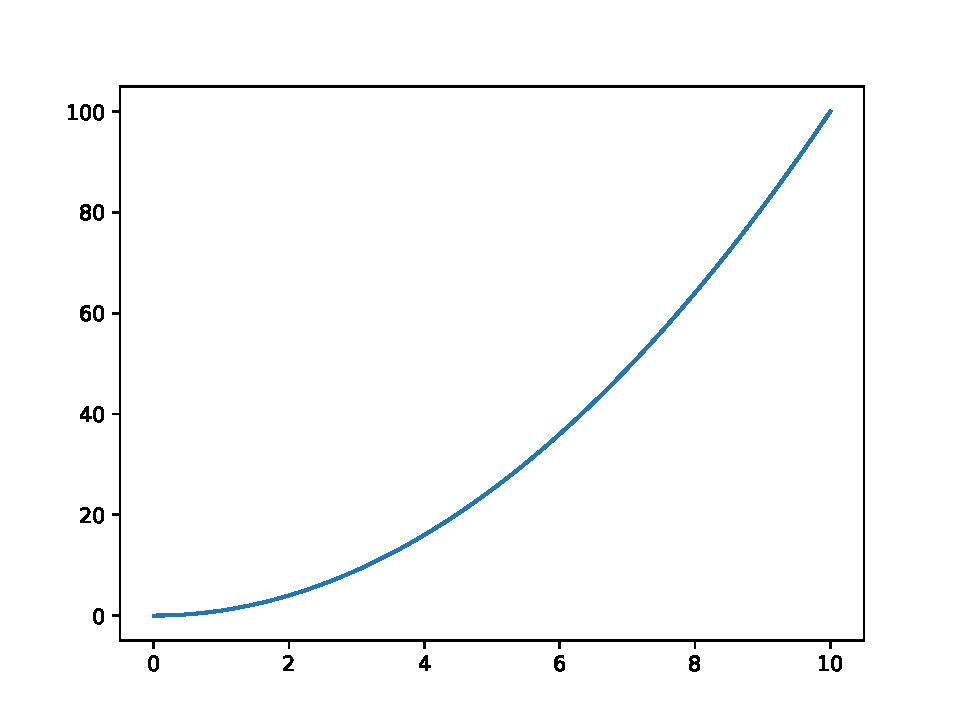
\includegraphics[width=0.8\textwidth]{x_squared}
\caption{\label{fig:x2} The result of the simple plotting script of $y = x ^ 2$.}
\end{figure}
%

The example above is rather simplistic, but the \texttt{matplotlib} library can be used to make very complex plots.
Furthermore, the example above would not perform well for experimental data, considering that the axes have no labels, the data is described with a line instead of points and there is no plot title.
However, the code below shows some realistic experimental data plotted using matplotlib in a fashion that is more comprehensible.
The plot produced can be found in Figure~\ref{fig:real},
\begin{lstlisting}
# Plotting some real data
import numpy as np
import matplotlib.pyplot as plt

temperature = np.linspace(283, 363, 10)
rate_constants = np.array([3.2e-19, 3.4e-18, 3.2e-17, 2.6e-16, 1.8e-15, 1.2e-14, 7.3e-14, 3.9e-13, 1.9e-12, 8.9e-12])
rate_constants_uncertainty = np.array([1.6e-20, 1.7e-19, 1.6e-18, 1.3e-17, 9.4e-17, 6.2e-16, 3.7e-15, 2.0e-14, 1.0e-13, 4.4e-13])

plt.errorbar(temperature, rate_constants*10**12, rate_constants_uncertainty*10**12, marker='o', linestyle='')
plt.ylabel(r'Rate constant/$\times10^{-12}$ s$^{-1}$')
plt.xlabel(r'Temperature/K')
plt.title(r'Effect of temperature of rate constant of HI decomposition')
plt.tight_layout()
plt.show()
\end{lstlisting}
%
\begin{figure}[t]
\centering
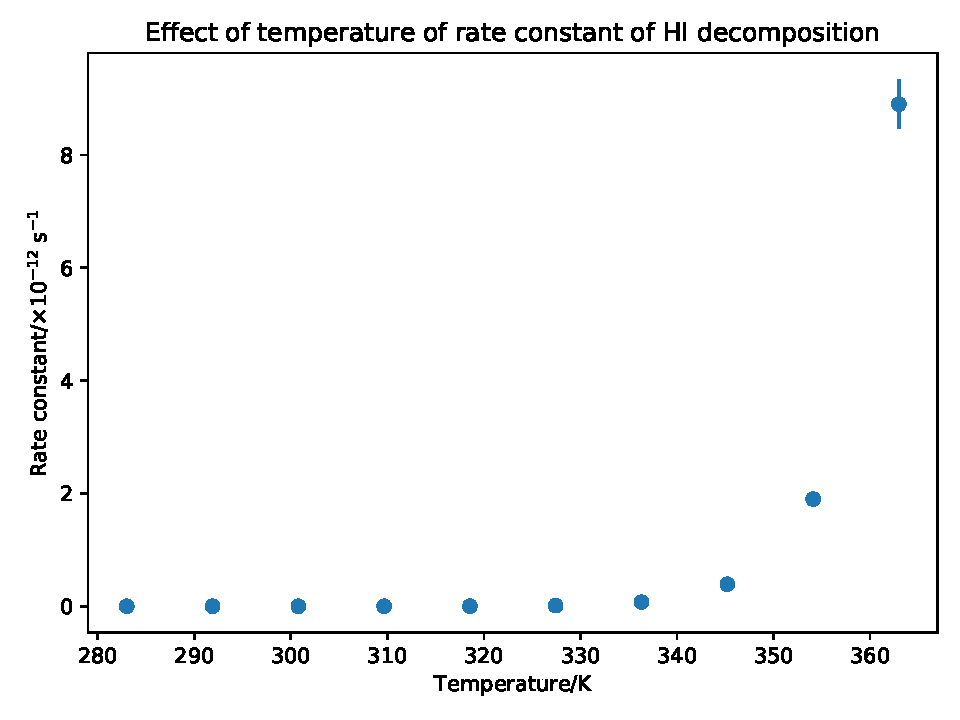
\includegraphics[width=0.8\textwidth]{real}
\caption{\label{fig:real} The result of the simple plotting script of $y = x ^ 2$.}
\end{figure}
%
\vspace{\baselineskip}
\begin{center}
	\noindent\fbox{%
		\begin{minipage}{0.9\textwidth}%
			\vspace{0.15\baselineskip}
			\subsubsection*{Exercise}
			\begin{itemize}
				\item{Read through the code used to plot the more ``realistic'' plot and determine what each element in the code does. Annotate this worksheet and ask a demonstrator to check you have all of the elements.}
			\end{itemize}
		\end{minipage}
	}
\end{center}

\section{Reading in data}

A lot of computational work in science involves processing data that has already been generated, either from a previous calculation or from an experiment. Entering data by hand (e.g.\ using \texttt{input()} is tedious, time-consuming, and error-prone.) If the data is already stored in a file, we would like to read this file directly.

The NumPy library includes the \texttt{loadtxt()} function, which will read a file containing columns of numbers and store the values as a NumPy array, making it easy to then do any subsequent analysis.
The \texttt{loadtxt()} function can take a number of additional arguments to help with parsing files formatted in specific ways\footnote{The \texttt{loadtxt()} documentation can be found at \url{https://docs.scipy.org/doc/numpy/reference/generated/numpy.loadtxt.html}.}.

The simplest example is if we have a file (called \texttt{myfile.txt}) that contains two rows of numbers separated by spaces. This can be read in using
\begin{lstlisting}
# Reading in some text

a = np.loadtxt('myfile.txt')
\end{lstlisting}
This creates a $(2\times N)$ two-dimensional NumPy array \texttt{a} (similar to a nested list). \texttt{a[0]} contains the first row of values from the file, and \texttt{a[1]} contains the second row of values.

Experimental datasets are often stored as \emph{columns} of data, instead of rows. A common filetype that uses column-formatting is the \texttt{.csv} ``comma-separated values'' format\footnote{The \texttt{.csv} format is popular for storing experimental data because it can be read directly into Microsoft Excel.}. The ``standard`` format for a \texttt{.csv} file is for the columns of data to be separated by commas (hence the name), but any characters can be used to separate, or \emph{delimit}, the columns, including whitespace (tabs or spaces).

Reading a \text{.csv} using \texttt{loadtxt()} requires us to supply some additional arguments:
\begin{lstlisting}
# Reading in a csv file

a = np.loadtxt('myfile.csv', delimiter=',', unpack=True)
\end{lstlisting}
In this example, we pass two extra optional arguments to the function, \texttt{delimiter} defines the character that separates the values in the columns, and \texttt{unpack} indicates that the data is stored in columns rather than rows.

Data files often include comments, used to explain how and when the data were collected, and to explain what each column of numbers represents. Providing comment lines start with a \texttt{\#} symbol, then \texttt{loadtxt()} automatically will ignore the line.

\section{Problems}

\subsection{Interatomic distances}

Write code that can take the $x$, $y$, and $z$ coordinates of three atoms and calculate the distances $r_{ij}$ between each pair. For each pair of atoms, print the interatomic distance.

The equation for the distance $r_{ij}$ between two atoms $i$ and $j$ is,
\begin{equation}
	r_{ij} = \sqrt{(x_i - x_j)^2 + (y_i - y_j)^2 + (z_i - z_j)^2}.
\end{equation}

\textbf{Remember}: Plan the structure of your program  before you start to write any code.

Download the \texttt{molecule1.txt} and \texttt{molecule2.txt} files from Moodle\footnote{Can be found in the Molecules folder.}, and copy these into your working directory (e.g.\ \texttt{H:/CH40208/week2}. Each file contains three columns, labelled $x$, $y$, and $z$, which you can read the atomic coordinates from. To calculate the distances between each pair of atoms you will need to use a pair of \emph{nested} loops. What do these distances tell you about the shapes of these molecules?

\textbf{Extension}: Using the Cosine rule,
%
\begin{equation}
  a^2 = b^2 + c^2 -2bc\cos(A),
\end{equation}
%
where the angles and distances are given in Figure~\ref{fig:cosine}, calculate the molecular angles $\theta_{ijk}$, and identify these molecular species.
%\begin{enumerate}
%	\item{Atom 1: ($0.1$, $0.5$, $3.2$); Atom 2: ($0.4$, $0.5$, $2.3$); Atom 3: ($-0.3$, $0.3$, $1.7$)}
%	\item{Atom 1: ($-0.1$, $0.5$, $1.5$); Atom 2: ($0.2$, $0.5$, $2.6$); Atom 3: ($0.5$, $0.5$, $3.7$)}
%\end{enumerate}
%
\begin{figure}[t]
\centering
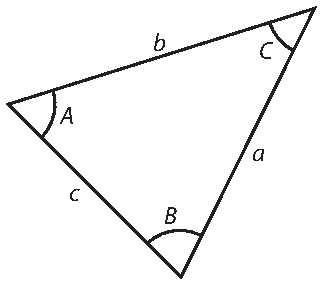
\includegraphics[width=0.4\textwidth]{triangle}
\caption{\label{fig:cosine} Guide for angles and distances when using the cosine rule.}
\end{figure}
%

\subsection{Optimisation}
This problem can be solved using simpler (and faster) code using NumPy arrays. Rewrite your code from the problem to use arrays and compare your results to your original version (you should get the same results). You might need to reconsider your algorithm to decide how to best use arrays to solve this problem.

\bibliographystyle{rsc}
\bibliography{handout_2}

\end{document}
